%
% einleitung.tex -- Beispiel-File für die Einleitung
%
% (c) 2020 Prof Dr Andreas Müller, Hochschule Rapperswil
%
% !TEX root = ../../paper.tex
% !TEX encoding = UTF-8
%
\section{Geschichte\label{geostrophisch:section:geschichte}}
\kopfrechts{Geschichte}

Die Anfänge der numerischen Wettervorhersage gehen auf den britischen Mathematiker und Physiker \emph{Lewis Fry Richardson} (1881–1953) zurück (Abbildung~\ref{bild:portraitRichi}).
Schon in jungen Jahren entdeckte er sein Interesse an der Mathematik und wie man diese einsetzen kann um die Menschheit voranzubringen.
Er entwickelte eine neue spezielle Methode, um analytisch nicht lösbare Partielle Differentialgleichungen zu lösen. 
Besagte Methode wurde in einem Artikel veröffentlicht. 
In seinem Werk \cite{geostrophisch:wpbnp} (1922) formulierte Richardson als Erster die Idee, eine numerische Wettervorhersage durch das explizite Lösen eines physikalisch fundierten Gleichungssystems zu bestimmen.  
Damit legte er den theoretischen Grundstein für die moderne Wettermodellierung.
Für diese erste Vorhersage von 6 Stunden brauchte er etwa 6 Wochen Zeit für die Berechnungen.
Zudem wich diese auch noch weit von der Realität ab.
Warum das so war und warum seine Arbeit trotzdem so wichtig für heutige Wettervorhersagen ist, darauf gehen wir in den folgenden Kapiteln ein. 
%Auch noch weiter an der Geschichte 
% Wie Buch verloren ging muss noch rein

\begin{figure}[h]
	\centering
	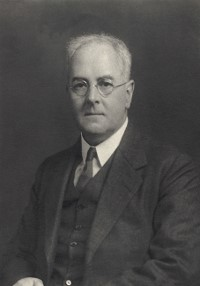
\includegraphics{Portrait_Richardson.jpg}
	\caption{Lewis Fry Richardson, 1881-1953, Autor des Buches \cite{geostrophisch:wpbnp} und damit Begründer }
	\label{bild:portraitRichi}
\end{figure}

\begin{itemize}
	\item \textbf{Bewegungsgleichungen:} Horizontale und vertikale Impulsbilanz
	\item \textbf{Kontinuitätsgleichung:} Erhaltung der Masse
	\item \textbf{Energiegleichung:} Thermodynamische Prozesse
	\item \textbf{Zustandsgleichung:} Zusammenhang zwischen Druck, Temperatur und Dichte
\end{itemize}






